% using Elseveir template per https://www.elsevier.com/authors/author-schemas/latex-instructions
\documentclass[review]{elsarticle}
\usepackage{lineno,hyperref}
\modulolinenumbers[5]
\bibliographystyle{elsarticle-num}

\usepackage{booktabs}
\usepackage{graphicx}
\graphicspath{{../alt-ed-survey/figures-and-tables}}
\usepackage{hyperref}
\usepackage{threeparttable}  
\usepackage{tikz}
\usetikzlibrary{calc,matrix}

\begin{document}
\begin{frontmatter}

    \title{
        COVID-19 and Alternative Postsecondary Learning
        % \tnoteref{titlenotes}
    }
    % \tnotetext[titlenotes]{
    %     Go to \url{https://github.com/Vandivier/research-dissertation-case-for-alt-ed/tree/master/papers/alt-ed-survey}
    %     for additional materials including the online appendix,
    %     survey data, and data analysis source code.
    % }

    \author[mymainaddress]{John Vandivier}
    \address[mymainaddress]{4400 University Dr, Fairfax, VA 22030}
    \ead{jvandivi@masonlive.gmu.edu}
    % \fntext[authorlinefootnote]{
    %     Vandivier: George Mason University,
    %     4400 University Dr, Fairfax, VA 22030,
    %     jvandivi@masonlive.gmu.edu.
    % }

    \begin{abstract}
        As a result of the coronavirus pandemic,
        many individuals now engage in remote activities that they would otherwise not.
        While other research has assessed the impact of coronavirus on K-12 education,
        this paper fills a gap in the literature regarding
        the impact to professional certifications and other unaccredited postsecondary credentials.
        This paper investigates the results of an original online questionnaire (n=350)
        to understand the effects of COVID-19
        on support for alternative postsecondary learning.
        Respondents are U.S. citizens over the age of 18.
        Cross-sectional analysis using ordinary least squares (OLS)
        and Iteratively Reweighted Least Squares (IRLS)
        indicates that individual perception of a large negative impact from coronavirus
        is significantly correlated with
        higher favorability to alternative credentials.
        Some important industrial, ethnic, and state effects are also identified.
        Independent factors including the level of education, income, age, and gender were identified as insignificant.
    \end{abstract}

    \begin{keyword}
        education economics, alternative education, coronavirus             %%% not grammatical
        \MSC[2010] I21, I22, J20 % Unused at AEL: D12, J23, I24, I25, I26   %%% not grammatical
    \end{keyword}

\end{frontmatter}

\pagebreak
\linenumbers

\section{Introduction}

This study is concerned with postsecondary alternative credentials.
This category includes professional certifications, coding bootcamps, portfolios of work, and other proof of education other than traditional credentials.
Traditional credentials include a high school diploma or an accredited degree from a university.
Many alternative credentials are obtained as a result of education that involves a substantial component of remote learning.
This study tests the hypothesis that the impact of coronavirus is associated with increased favorability toward alternative credentials.
% This study also examines whether coronavirus-induced remote activity is associated with favorability to alternative credentials.
Results favor the hypothesis, with a few interesting caveats.

There are three theoretical reasons to suppose that a pandemic would make alternative postsecondary credentials more attractive.
The first is that a pandemic would induce increased remote learning.
This causes exposure, and exposure effects are generally positive on favorability.
Secondly, alternative learning providers tend to be smaller, less regulated, and better able to adapt in the face of social change
compared to the traditional postsecondary provider of education, the accredited university.
% As a result, alternative learning providers will adapt more quickly during a pandemic.
In the face of a pandemic, comparatively higher quality at a lower price is expected by alternative producers,
and high comparative consumer favorability would be expected to follow.

The third theory is that a pandemic is a time when normal strangeness increases across society.
When the normal level of strangeness increases, things which were already finitely strange become relatively less strange.
Alternative credentials are strange in some sense by construction,
but the relative stigma associated with these credentials might decrease in a time of pandemic.
This becomes more plausible when the connection of alternative credentials to remote activity is highlighted.
At a time when personal contact is costly,
remote learning becomes a better bargain,
and the social benefits of traditional education are simultaneously diminished.

% This would theoretically reduce any relative stigma which the alternatively educated invididual might face.
% The stigma is reduced by two mechanisms.
% First, society changes many norms during a pandemic, so the general strength of social norms is reduced.
% In this way, the general preference for traditional over alternative education is reduced.
% Secondly, consuming alternative education is specifically reasonable as a pandemic adaptation.
% During a pandemic, many of the attractions of university life are unusable,
% remote learning provides protection against becoming ill,
% and pinching pennies is more understandable than it is during times of flourishing.
% When an individual has such good reasons for pursuing alternative education, it becomes unreasonable to impose a stigma at hiring decision time.
% TODO: the above is related to mitigation tactics for disabled people during interview; stigma management...idk the exact keywords look it up

% The third reason that a pandemic could make a massive shift to alternative learning more reasonable
% is simply that massive shifts are less spectacular in a time of pandemic.
% Society has already changed many norms in the face of the pandemic.
% Some of these norm changes are directly linked while others are indirect.
% Social distancing, wearing masks, fewer shaken hands, and so on, are some direct measure.
% The lack of fresh bread at my local coffee shop is an indirect change resulting from supply chain cost impact of the pandemic.
% Both are understandable changes.
% In this pandemic context an empathetic employer would look at an alternatively educated individual as making a reasonable adaptation,
% whereas previously they might face some stigma for making a strange choice.
% In a time where many norms are being disrupted, there may be an external effect which weakens norms in general,
% and therefore the general preference of traditional to alternative education would.

While exposure to some stigma generally increases favorability, there are several special cases where it declines instead.
It could be the case that coronavirus-induced remote learning and work are an exceptional case where decline is observed.
This paper is valuable in part because it replaces this ambiguity with empirical evidence.
Pandemic exposure is an interesting case of exposure because it is a harmful, unwanted, or forced exposure.
It is not clear that coronavirus-induced exposure to remote learning and work will result in
Remote work and learning which are taken as a result of the pandemic might be perceived negatively by association,
or they might be perceived as a useful option that becomes more valuable in light of an unfortunate pandemic.
% TODO: cite these biases
Familiarity bias and mere-exposure effects are generally positive on favorability to some stimulus,
but these exposures are generally voluntary. Unwanted exposure can generate positive or negative favorability changes,
and when the exposure involves harm it tends to reduce favorability.
Backfire, boomerang, and blowback effects are some examples of negative favorability reactions to exposure.
One study hits remarkably close to COVID-19 pandemic relevance because it found a backfire effect in efforts to market flu vaccine usage,
unintentionally resulting in reduced willingness to take the flu vaccine [1].
Even repeated unwanted exposure to harm can eventually lead to positive favorability through as documented in the work on Stockholm syndrome.

The actual effect of coronavirus could mimick a combination of the above effects.
As a result, it is not obvious a priori whether the actual effect is positive, negative, or insignificant,
and this ambiguity calls for empirical investigation.
Individual favorability to alternative credentials is also like to vary for a variety of personal reasons which are unrelated to the pandemic.
This paper uses multiple regression to identify the net effect of coronavirus on favorability while holding constant these other sources of variation.

% [1] https://www.theatlantic.com/health/archive/2014/12/vaccine-myth-busting-can-backfire/383700/
% https://pubmed.ncbi.nlm.nih.gov/15974346/
% https://en.wikipedia.org/wiki/Belief_perseverance

There are already several papers examining the impact of coronavirus on the education system.
These papers focus on education from kindergarten through high school,
but it is reasonable to expect postsecondary education to be impacted in a similar way.

% TODO: cite four papers and show how they relate
% TODO: why do we care about these credentials? 1 higher quality, 2 lower price, 3 faster, 4 align to workforce needs, 5 solve for equity/equality
% TODO: alt creds vs alt ed? signalling theory says credentials communicate value;
%       from a modeling perspective they make alt ed concrete by demarking achievement for factor attribution
% TODO: BLS data: "postsecondary nondegree award"
% TODO: other orgs? saylor academy, lumina foundation, credly/acclaim, ACE gov body, (OER) open ed resources much online, 'skill gap'
% TODO: why remote learning matters? even traditional is moving that way

\section{Description of Data and Methodology}

This paper uses an original set of response data (n = 350) obtained through the administration of an online questionnaire.
This cross-sectional data was obtained at the beginning of February in 2021.
Respondents are United States citizens at or over the age of eighteen.
The Amazon Mechanical Turk platform was used to recruit qualified participants.

Responses are investigated using regression analysis and descriptive statistics including skew
\footnote{
    While the data for this analysis is not public, the analytical code is open-source.
    See \url{https://github.com/Vandivier/research-dissertation-case-for-alt-ed/tree/master/papers/alt-ed-covid-2/data}
}.
% Mild skew was detected, so results of interest are compared with and without skew correction.
% Adjustments for skew constrain the applicability of results.
Regression analysis includes multiple regression of linear and curvilinear effects
with either ordinary or robust linear modelling.
Ordinary linear modelling uses ordinary least squares,
and robust linear modelling (RLM) uses iteratively reweighted least squares.
% TODO: paper showing why use a robust linear model and/or that it's a good practice to compare to OLS
Factor coefficients across these approaches are comparable,
but RLM does not generate a useful R-squared statistic
for model-level comparison.

Appendix A contains the exact wording and response options for each question.
Appendix A also contains the wording for a priming message presented at the start of the survey.
The priming message lays out the definition of alternative credentials for the purposes of the study.
The message also provides several concrete examples of alternative credentials,
including "a Certified Project Manager certification,
a portfolio of work, a Khan Academy profile, or a Nanodegree from Udacity."

The questionnaire is composed of fourteen questions.
There is one for the dependent variable of interest, favorability,
one for the independent variable of interest, coronavirus impact,
ten control factors,
and two questions on causality.

% TODO: cite a couple papers
Eight of the ten control factors are common controls in the literature.
These eight controls are categorical measures for
for age, gender, ethnicity, income,
level of education, employment status, industry of occupation, and state of residence.

The two remaining controls are unique to this study.
The first is expectated conventionality.
This is question three in the appendix.
This control is meant to explain the favorability effect attributable to the normative acceptability of alternative credentials.
This allows the favorability effect to be interpreted along simple lines of individual favorability,
holding constant an important side-question about the way social norms relate to individual favorability.
% As a matter of current social norms, alternative credentials are stigmatized when treated as a substitute for the traditional degree.

% TODO: maybe talk about a couple papers that say mode of instruction is related to favorability
The second unique control is support for online education.
This is question four in the appendix.
This control allows an analyst to hold constant the mode of instruction when interpreting favorability to alternative credentials.
% Mode of instruction is a bit of a red herring which is not what this study is centrally concerned with.
% Favorability to online education creates noise in the signal of favorability to alternative credentials,
% and this factor seperates that effect.
% The reason isolating this noise is important is because there are two assumptions in the mind of the respondent population.
% The first assumption is that traditional education involves in-person learning.
% The second assumption is that alternative education typically involves remote learning.
% Neither of these associations are held as true in the current analysis, so the introduction of this control allows
% Alternative education often employs remote learning, but this is not always the case.
% A respondent may still tend to associate the concepts and impute a halo effect from one to the other.
% This control allows an analyst to seperate favorability from alternative credentials

The primary interest of this study is to identify the effect or lack of effect of coronavirus on favorability.
If an effect is found, however, an interesting question arises on the mechanism which supports that effect.
Both unique controls and the two questions on causality support this investigation about mechanism.
Specifically, one hypothesized mechanism is that coronavirus stimulates remote activity,
then exposure to remote activity improves favorability to all remote activities,
then alternative credentials improve in favorability through a normative association with remote learning.

The variables of interest,
causality questions,
and the two unique controls obtain Likert-type responses.
The impact of coronavirus and the causality questions use a 4-point scale.
Favorability and the unique controls use a 10-point scale.
Continuous treatment of items on the 10-point scale permits curvilinear analysis,
including investigation of interesting marginal effects
\footnote{
    It is an accepted practice to treat Likert-type responses as either categorical or continuous for regression analysis.
    Jaccard and Wan provide support for continuous analysis of Likert-type data.
    They note that severe departures from the assumptions on cardinality "do not seem to affect Type I and Type II errors dramatically,"
    particularly when the Likert scale is five or more points\cite{jaccard1996lisrel}.
    This paper treats responses on a 10-point scale as continuous.
    This paper treats responses on a 4-point scale as categorical.
}.

\section{Results}

The median favorability response was eight out of ten.
Figure \ref{fig:one} visualizes the distribution of responses.
Of 350 responses, 11 responses indicate a favorability of less than four out of ten.
Regression analysis indicates a significant and positive coronavirus impact effect,
invariant to whether outliers are dropped.
% As a conservative interpretation,
The effect of the coronavirus impact on favorability
is not held with confidence over the outlier range.

\begin{figure}[h!]
    \centering
    \caption{Distribution of Favorability to Alternative Credentials}
    \begin{tikzpicture}[element/.style={minimum width=1.75cm, minimum height=0.85cm}]
        \node (n1) {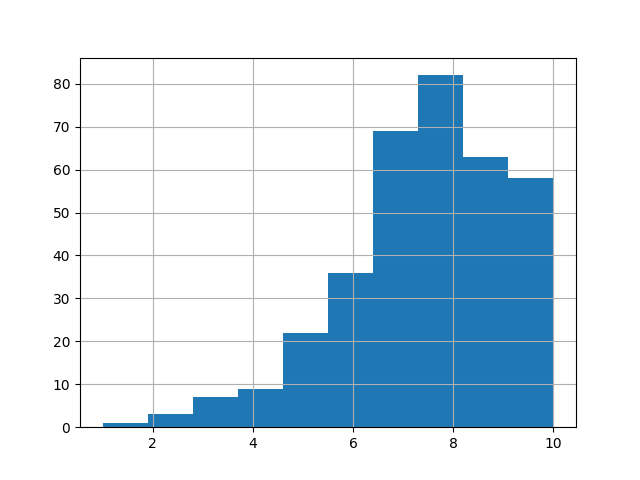
\includegraphics[width=0.7\textwidth]{./figures-and-tables/figure-1.png}};
    \end{tikzpicture}
    \label{fig:one}
\end{figure}

The average response was 7.65 on a 10-point scale.
Excluding outliers, over 96 percent of responses fall into the normal range.
The average response in the normal range was about 7.81.
Table \ref{tab:desc_stats} summarizes statistics about favorability,
the direct measure of coronavirus impact,
and the two support factors about the mechanism of coronavirus impact.

Summary statistics are given for the total population and three subpopulations.
The subpopulations include the normal range, the outlier population, and the Tens.
Because factors in Table \ref{tab:desc_stats} dummy variables,
with an exception for favorability,
the mean values for each variable can be interpreted as the proportion of the population
that affirms the response.

The Tens are those individuals that responded with a favorability of 10 to alternative credentials.
This is not an outlier group, but they are interesting to allow a better understanding of the distribution of responses.
These groups are in some ways similar to each other and in other ways they are importantly different.
For example, there are no negative outliers that report a large perceived impact from coronavirus.
In contrast, the Tens report a large perceived impact at a disproportionately high rate.
This is important when conclusions about the American population are drawn from the discussion on factor effects.

This data is consistent with external reporting that most Americans are impacted by coronavirus\cite{demographic2020},
but it adds the wrinkle that most Americans consider the impact to be minor.
This is another case where outliers and Tens importantly differ from the average.
The Tens report higher coronavirus impact while the outliers cluster around a medium impact response.

\begin{table}
    \caption{Summary Statistics for Factors of Interest}
    \resizebox{\columnwidth}{!}{
        {
\def\sym#1{\ifmmode^{#1}\else\(^{#1}\)\fi}
\begin{tabular}{llcc}
    \toprule
                              &                                   & \textbf{Average Hirability} & \textbf{Average Prestige} \\
    \midrule
    \textbf{Actual Schools}   &                                   &                             & 6.50                      \\
                              & \textbf{Accredited}               &                             & 7.05                      \\
                              & \textbf{Unaccredited}             &                             & 6.07                      \\
                              & \textbf{Difference}               &                             & 0.98                      \\
    \cmidrule{2-4}
                              & \textbf{Stipulated High Prestige} &                             & 6.72                      \\
                              & \textbf{Stipulated Low Prestige}  &                             & 6.23                      \\
                              & \textbf{Difference}               &                             & 0.49                      \\
    \cmidrule{2-4}
    \textbf{Vignette Schools} &                                   & 6.49                        & 6.21                      \\
                              & \textbf{Accredited}               & 6.97                        & 6.49                      \\
                              & \textbf{Unaccredited}             & 6.02                        & 5.93                      \\
                              & \textbf{Difference}               & 0.95                        & 0.56                      \\
    \cmidrule{2-4}
                              & \textbf{Stipulated High Prestige} & 7.59                        & 7.69                      \\
                              & \textbf{Stipulated Low Prestige}  & 5.63                        & 4.94                      \\
                              & \textbf{Difference}               & 1.96                        & 2.75                      \\
    %   \midrule
    % \textbf{Pooled}           &                                   &                             & 6.37                      \\
    %                           & \textbf{Accredited}               &                             & 6.77                      \\
    %                           & \textbf{Unaccredited}             &                             & 6.01                      \\
    %                           & \textbf{Difference}               &                             & 0.76                      \\
    %                           & \textbf{Stipulated High Prestige} &                             & 7.00                      \\
    %                           & \textbf{Stipulated Low Prestige}  &                             & 5.80                      \\
    %                           & \textbf{Difference}               &                             & 1.20                      \\
    \bottomrule
    \bottomrule
\end{tabular}
}

    }
    \label{tab:desc_stats}
\end{table}

Table \ref{tab:multiple_regs} provides factor coefficients for four interesting OLS models.
Model 1 is the adjusted R-squared maximizing model.
Model 4 is composed only of significant factors.
Model 2 is Model 4 plus a dummy for a large coronavirus impact.
Model 3 follows the same specification as Model 2,
but it is assessed against the normal range of the population, excluding outliers.

\begin{table}
    \caption{Table of Multiple Regressions}
    \resizebox{\columnwidth}{!}{
        {
\def\sym#1{\ifmmode^{#1}\else\(^{#1}\)\fi}
\begin{tabular}{lcccccc}
\toprule
                                                   & \textbf{coef} & \textbf{std err} & \textbf{t} & \textbf{P$> |$t$|$} & \textbf{[0.025} & \textbf{0.975]}  \\
\midrule
\textbf{Intercept}                                 &       3.4814  &        0.431     &     8.071  &         0.000        &        2.633    &        4.330     \\
\textbf{conventional\_alt\_creds}                  &       0.4485  &        0.045     &     9.918  &         0.000        &        0.360    &        0.537     \\
\textbf{favor\_online\_ed}$^2$                     &       0.0993  &        0.035     &     2.843  &         0.005        &        0.031    &        0.168     \\
\textbf{covid\_ind\_remote\_large\_degree}         &       0.5613  &        0.206     &     2.721  &         0.007        &        0.156    &        0.967     \\
\textbf{covid\_ind\_fav\_online\_large\_degree}    &      -0.8037  &        0.309     &    -2.602  &         0.010        &       -1.411    &       -0.196     \\
\textbf{covid\_ind\_fav\_online\_moderate\_degree} &      -0.6581  &        0.243     &    -2.711  &         0.007        &       -1.136    &       -0.181     \\
\textbf{covid\_ind\_fav\_online\_slight\_degree}   &      -0.5347  &        0.251     &    -2.127  &         0.034        &       -1.029    &       -0.040     \\
\textbf{industry\_health}                          &       0.5461  &        0.288     &     1.894  &         0.059        &       -0.021    &        1.113     \\
\textbf{industry\_information\_technology}         &       0.3394  &        0.192     &     1.766  &         0.078        &       -0.039    &        0.717     \\
\textbf{industry\_manufacturing}                   &       0.6792  &        0.294     &     2.307  &         0.022        &        0.100    &        1.258     \\
\textbf{industry\_real\_estate}                    &       1.1427  &        0.645     &     1.770  &         0.078        &       -0.127    &        2.412     \\
\textbf{ethnicity\_hispanic}                       &       0.7559  &        0.414     &     1.827  &         0.069        &       -0.058    &        1.570     \\
\textbf{ethnicity\_other}                          &       1.5186  &        0.781     &     1.945  &         0.053        &       -0.017    &        3.054     \\
\textbf{ethnicity\_white\_caucasian}               &       0.4370  &        0.180     &     2.432  &         0.016        &        0.083    &        0.791     \\
\textbf{state\_georgia}                            &       1.2169  &        0.509     &     2.392  &         0.017        &        0.216    &        2.218     \\
\textbf{state\_iowa}                               &      -2.6606  &        0.882     &    -3.018  &         0.003        &       -4.395    &       -0.926     \\
\textbf{state\_kentucky}                           &      -1.2358  &        0.682     &    -1.812  &         0.071        &       -2.577    &        0.106     \\
\textbf{state\_ohio}                               &      -1.3443  &        0.638     &    -2.108  &         0.036        &       -2.599    &       -0.090     \\
\textbf{state\_pennsylvania}                       &      -0.9913  &        0.468     &    -2.116  &         0.035        &       -1.913    &       -0.070     \\
\bottomrule
\end{tabular}
% \end{center}
% \begin{center}
% \begin{tabular}{lclc}
% \toprule
% \textbf{Omnibus:}       & 23.897 & \textbf{  Durbin-Watson:     } &    2.218  \\
% \textbf{Prob(Omnibus):} &  0.000 & \textbf{  Jarque-Bera (JB):  } &   29.746  \\
% \textbf{Skew:}          & -0.558 & \textbf{  Prob(JB):          } & 3.47e-07  \\
% \textbf{Kurtosis:}      &  3.892 & \textbf{  Cond. No.          } &     124.  \\
% \bottomrule
% \end{tabular}
}

    }
    \label{tab:multiple_regs}
\end{table}

The direct effect of coronavirus appears to be weak but positive.
The response indicating that a person has perceived a large impact from coronavirus was the only factor to appear in these models of interest.
Notice that the large impact factor is invariant to the outlier subpopulation,
because no negative outlier reported a large impact.

The two causality questions are significant across models.
The coefficients range from half a point to a point, which indicates moderate importance.
The first causality question asks whether coronavirus caused an increased degree of remote activity for the respondent.
The coefficient on the dummy variable indicating a large coronavirus-induced increase to remote activity is positive.
This is consistent with the hypothesis of a positive exposure effect.

The second question on causality asks whether coronavirus-induced remote activity has caused an increase
to favorability to remote learning.
The exact wording is:
"To what degree has coronavirus-induced remote activity improved your favorability to remote learning
(either for yourself or for other people)?"
As such, any response other than "none" constitutes evidence that coronavirus caused increased favorability to remote learning.
Given that there is a positive relationship between favorability to online learning and favorability to alternative credentials,
any response other than "none" effectively supports the hypothesized mechanism in which an exposure effect leads to support for alternative credentials.
Referring back to Table \ref{tab:desc_stats},
about 83.1 percent of the full population of Americans indicate a small,
medium, or large increase to favorability of remote learning
caused by coronavirus-induced remote activity.

The observation of nonzero responses to the factor for coronavirus-induced remote learning favorability is causal evidence.
The fact that these nonzero responses are negatively related to favorability is a non-causal association.
This association indicates that those who gained the most in favorability also ended with less than average favorability.
This means the greatest gainers started far below the average and ended slightly below the average,
while those with prior high favorability did not move much higher.
This interpretation is reinforced by referring back to the summary statistics in Table \ref{tab:desc_stats}.
Notice that the negative outlier group has highest affirmative response with respect to both a
medium increase to remote favorability
and also to a large increase to remote favorability.
The normal range, on the other hand, has the highest indication of a small increase to remote favorability.
This makes sense given that the median response is already near the maximum response.

Coronavirus-induced favorability to online education is distinct from a plain measure of favorability to online education.
The latter is labeled Favor Online Education within Table \ref{tab:multiple_regs},
and it is one of the two unique controls discussed in the Methodology.
This factor was most significant when modeled as a quadratic term.
The positive coefficient on the quadratic term can be interpreted as a positive marginal effect over the sample range.
It is worth noting that plain favorability to online education
and coronavirus-induced favorability to online education share a nontrivial correlation (Pearson's $r=0.303$).
This demonstrates internal consistency among responses and it also further validates the explanation from exposure.

The other unique control is expected conventionality.
This factor is also significant, robust to specification, and important.
Expected conventionality is moderately correlated with favorability to online education (Pearson's $r=0.445$),
but it is uncorrelated to coronavirus-induced favorability to online education.
This indicates that respondents do not seem to generate a greater expectation that alternative credentials will be conventional in the future
after being exposed to coronavirus-induced remote activity.

Table \ref{tab:table_robust_reg} is a table of factors for a robust linear model (RLM).
Robust regression is useful in part to address samples in which outliers exist, so the whole sample is used.
Because RLM enters factors in linearly, the coefficients are comparable to OLS coefficients.
This makes the model in Table \ref{tab:table_robust_reg} useful for factor analysis as well.
Specifically, the model in this table is a simple respecification of Model 4 from Table \ref{tab:multiple_regs} into RLM.
The main result in this table is that none of the effects of interest are importantly different between RLM and OLS specification.

\begin{table}
    \caption{Table of Factors for Robust Linear Model}
    \resizebox{\columnwidth}{!}{
        {
\def\sym#1{\ifmmode^{#1}\else\(^{#1}\)\fi}
\begin{tabular}{lcccccc}
    \toprule
                                                    & \textbf{coef} & \textbf{std err} & \textbf{z} & \textbf{P$> |$z$|$} & \textbf{[0.025} & \textbf{0.975]} \\
    \midrule
    \textbf{Favor Online Education$^2$}             & 0.1083        & 0.033            & 3.289      & 0.001               & 0.044           & 0.173           \\
    \textbf{Expected Conventionality}               & 0.4566        & 0.042            & 10.855     & 0.000               & 0.374           & 0.539           \\
    \textbf{Large Change to Remote Activity}        & 0.6981        & 0.192            & 3.637      & 0.000               & 0.322           & 1.074           \\
    \textbf{Small Increase to Remote Favorability}  & -0.6117       & 0.236            & -2.595     & 0.009               & -1.074          & -0.150          \\
    \textbf{Medium Increase to Remote Favorability} & -0.7676       & 0.228            & -3.362     & 0.001               & -1.215          & -0.320          \\
    \textbf{Large Increase to Remote Favorability}  & -0.8345       & 0.290            & -2.874     & 0.004               & -1.404          & -0.265          \\
    \textbf{Industry, Health}                       & 0.5969        & 0.271            & 2.205      & 0.027               & 0.066           & 1.128           \\
    \textbf{Industry, Information Technology}       & 0.4016        & 0.180            & 2.237      & 0.025               & 0.050           & 0.754           \\
    \textbf{Industry, Manufacturing}                & 0.7399        & 0.277            & 2.672      & 0.008               & 0.197           & 1.282           \\
    \textbf{Ethnicity, Caucasian}                   & 0.3168        & 0.161            & 1.963      & 0.050               & 0.001           & 0.633           \\
    \textbf{Ethnicity, Other}                       & 1.7074        & 0.724            & 2.359      & 0.018               & 0.289           & 3.126           \\
    \textbf{State, Georgia}                         & 1.0604        & 0.479            & 2.212      & 0.027               & 0.121           & 2.000           \\
    \textbf{State, Ohio}                            & -1.0150       & 0.601            & -1.690     & 0.091               & -2.192          & 0.162           \\
    \textbf{State, Pennsylvania}                    & -0.8238       & 0.441            & -1.867     & 0.062               & -1.688          & 0.041           \\
    \textbf{Intercept}                              & 3.5185        & 0.401            & 8.785      & 0.000               & 2.734           & 4.303           \\
    \midrule
    \textbf{N}                                      & 350           &                  &            &                     &                 &                 \\
    \bottomrule
\end{tabular}
}

    }
    \label{tab:table_robust_reg}
\end{table}

The other control variables also exhibit some interesting effects.
Caucasians disproportionately attend and graduate from college,
so this group is somtimes seen as a guard of the traditional degree or an opponent of alternative education. % TODO: citation
Alternative credentials are viewed as a diversity strategy,
and minority students do benefit disproportionately from alternative learning programs. % TODO: citation
This analysis presents evidence that undermines those narratives by observing a significant positive correlation between favorability and caucasian ethnicity.

Information Technology is a well-known bastion of alternative credentials including coding bootcamps.
This industry is fundamentally connected to the web and is unique in the high rate of obscolescence of dated learning.
It is not surprising that it is positively associated with favorability,
but it is surprising that it comes in third place among four industries with positive and significant favorability.

Health is an industry which has historically been difficult to digitize,
and it is sometimes given as an explicit example of an industry in which alternative credentials
might not work. % TODO: cite regulatory concerns and also cite improvements to simulation technology.
This analysis may indicate improvements to digital learning in health,
or changing social attitudes on whether accredited credentials are
generally preferred for many industry positions.

There are a variety of political and cultural reasons for which favorability might vary by state,
but no obvious explanation is evidenced in the current analysis.
Employment status was largely insignificant,
but Model 1 hints at a weak positive effect among hiring managers.
It is also interesting to note the control variables that are identified as insignificant.
Gender, age, and level of education had no bearing on favorability.
This provides weak evidence against the hypotheses that older individuals
or individuals that do have traditional degrees have a disproportionate opposition to alternative credentials.

\section{Conclusions}

% TODO: conclusion:
% 1. it's a bit speculative, but do we think this bump is transient or permanent? why?
% 2. how does this relate to covid impact to school choice results?
% 3. what open questions remain?
%     a. collecting more samples and samples over time would allow for more confidence bc multi-specification checks, forward-testing, more factor confidence.
%     b. identifying underlying patterns within-group for state, industry, and ethnic effects could prove useful for modelling and also instructive for policy.
%          i. my skill gap survey dives into industry effects.
%     c. alternative credentials are extremely diverse. a useful study would disaggregate this category and ask about alternative credentials of different kinds.
%          i. my prestige study does this, and the skill gap study to some degree.
% 4. are there any implications for consumers, policymakers, firms/hiring managers, or alternative education providers?

This study introduced controls for mental effort and personality into an estimate of favorability of alternative postsecondary learning.
The main hypothesis was that these controls would deflate an apparent paradox in conservative opposition to a market solution.
Contrary to expectation, the paradoxical pro-regulatory effect was amplified with significance.
Personality factors were identified with importance and contributed to superior model power.

Conscientiousness and openness were important Big Five traits.
Grit was independently important in a multiple regression over and above conscientiousness.
Individuals high in grit experienced weaker familiarity bias.

Robustness of the pro-regulatory effect may be explained using a combination of three alternative hypotheses.
First, the pro-regulatory effect may represent an unobserved logical structure.
This hypothesis makes sense of improved effect identification resulting from added controls.
This hypothesis also makes sense of the lack of important mental effort effects.

A second hypothesis is that the measure of status quo bias is ineffective.
This explanation holds that status quo bias in education is particularly strong.
After correcting for the status quo proxy, there could be residual status quo bias remaining in the estimate.

In this study, the favorability of artificial intelligence is used as an innovation proxy.
Low favorability is taken to indicate status quo bias.
As artificial intelligence becomes normal,
favorability tends to become a poor tool to distinguish innovation from the status quo.
It seems plausible that for some respondents,
artificial intelligence is less a deviation from the status quo
compared to unaccredited learning.

The hypothesis of proxy failure may dovetail with an explanation from an unobserved logical structure.
That is, some conservatives may carve out education as a logical-ideological exception to general market favorability.

A third hypothesis is that there is systematic variation in the sample.
This explanation leverages an unexpected difference in the favorability to artificial intelligence
in the current sample compared to prior periods.
This variation can be taken as random,
but it might also be attributable in part to a recent massive social adoption of new technologies.
COVID-19 has forced massive social change to technology use.
This may contribute to an unexpectedly rapid normalization of artificial intelligence.
This third hypothesis need not exclude some effect from the other two.

\bibliography{./BibFile}

\end{document}
